\section{Results}
%---------------------------------------------------------------------------------------------------
\subsection{Risk Group Duration}\label{res.yss}
Figure~\ref{fig:yss.fit} illustrates the distributions of
observed proportions $p_z$ \vs inferred proportions $\hat{\rho}_z$ of women
reporting durations $d_i \in \mathbb{d}_z$ selling sex,
following each stage of adjustment outlined in \sref{meth.yss}.
Figure~\ref{fig:yss.adj} illustrates
the estimated cumulative distributions for years selling sex following each stage of adjustment,
while Table~\ref{tab:yss.adj} provides the corresponding distribution means $\bar{D}$ and \ci.
Ironically, the final estimate of 4.06~(2.29,~6.34) is similar to the original median of 4,
as each adjustment alternates betwen increasing and decreasing $\bar{D}$.
The censoring adjustment yields the largest increase, while
the measurement adjustment yields the largest decrease.
\begin{figure}[h]
  \centering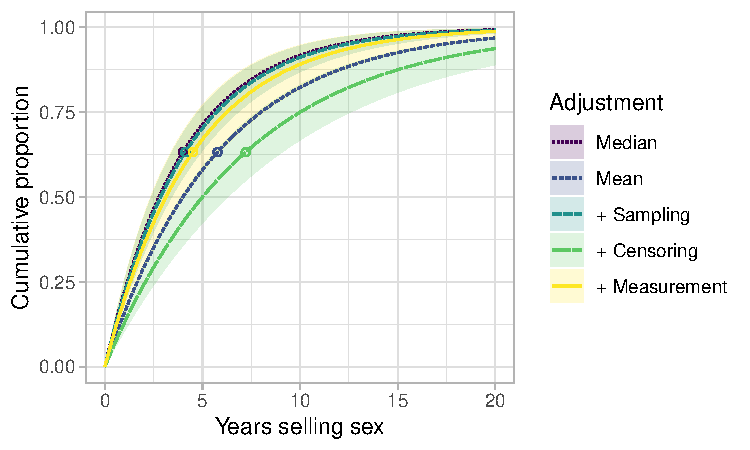
\includegraphics[scale=.75]{yss.adj}
  \caption{Estimated cumulative distribution for years selling sex
    following stages of adjustment}
  \label{fig:yss.adj}
  \floatfoot{Guide:
    \g{lines}{cumulative distribution under posterior mean},
    \g{shaded ribbon}{\ci},
    \g{circles}{posterior mean}.}
\end{figure}
%---------------------------------------------------------------------------------------------------
\subsection{Rates of Partnership Change}\label{res.parts}
Figure~\ref{fig:parts.fit} illustrates the distributions of
observed proportions $p_z$ \vs inferred proportions $\hat{\rho}_z$ of women
reporting $x_i \in \mathbb{x}_z$ partners in the past 30 days,
under the three partnership duration assumptions.
Figure~\ref{fig:parts.fsw} illustrates the inferred
rates of partnership change ($Q$) and numbers of current partners ($K$) under each assumption,
while Table~\ref{tab:parts.fsw} provides the corresponding means and \ci.
The biased estimates of $Q$ and $K$ appear equal because $Q$ is defined as per-month.
Biases are strongest for
$Q$ with long partnerships (\eg non-paying partners) and
$K$ with short partnership (\eg new clients).
However, biases are also substantial for
both $Q$ and $K$ with ``medium-length'' partnerships (\eg regular clients).
Figure~\ref{fig:parts.grid} illustrates generalized trends in these biases.
\begin{figure}
  \centering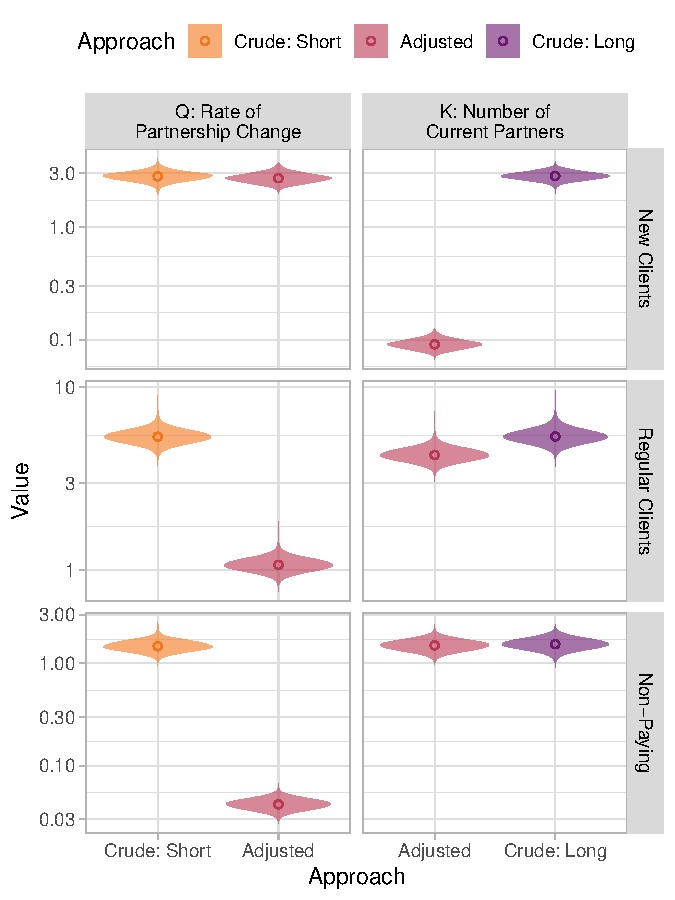
\includegraphics[scale=.75]{parts.fsw}
  \caption{Estimates of rates of partnership change and numbers of current partners
    under different partnership duration assumptions
    for three partnership types reported by female sex workers}
  \label{fig:parts.fsw}
  \floatfoot{Guide:
    \g{circles}{posterior mean},
    \g{shaded area}{posterior distribution}.
    Rates are per-month.}
\end{figure}
\begin{figure}
  \centering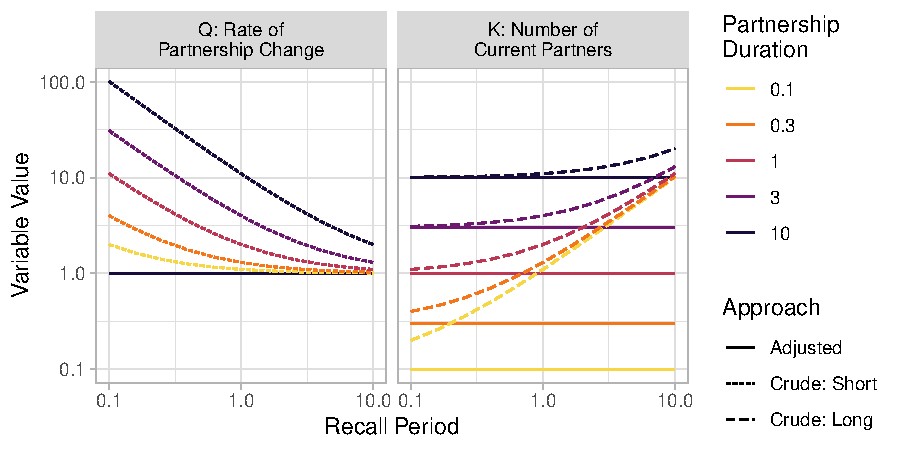
\includegraphics[scale=.8]{parts.grid}
  \caption{Estimates of rates of partnership change and numbers of current partners
    under different partnership duration assumptions
    for different recall periods and partnership durations}
  \label{fig:parts.grid}
  \floatfoot{Units are arbitrary.}
\end{figure}
